%\setcounter{figure}{-1}
%\setcounter{table}{-1}
%\setcounter{section}{-1}
\setcounter{NAT@ctr}{-1}

\articletitle{Development and evaluation of a culture-free microbiota profiling platform (MYcrobiota) for clinical diagnostics}
Stefan Boers\textsuperscript{\ref{affil:emc-microbiology},*},
Saskia Hiltemann\textsuperscript{\ref{affil:emc-bioinf},*},
Andrew Stubbs\textsuperscript{\ref{affil:emc-bioinf}},
Ruud Jansen\textsuperscript{\ref{affil:streeklabhaarlem}},
John Hays\textsuperscript{\ref{affil:emc-microbiology}}

\small
\begin{enumerate}
\itemsep-0.5em
\item Department of Bioinformatics, Erasmus Medical Center, Rotterdam, The Netherlands. \label{affil:emc-bioinf}
\item Department of Medical Microbiology and Infectious Diseases, Erasmus Medical Centre, Rotterdam, The Netherlands \label{affil:emc-microbiology}
\item Department of Molecular Biology, Regional Laboratory of Public Health Kennemerland, Haarlem, The Netherlands. \label{affil:streeklabhaarlem}
\end{enumerate}

{\color{chaptergrey}{Published in:}} European Journal of Clinical Microbiology \& Infectious Diseases \\
{\color{chaptergrey}{DOI:}} 10.1007/s10096-018-3220-z \\
{\color{chaptergrey}{*:}} Stefan A. Boers and Saskia D. Hiltemann contributed equally to this work.
% https://link.springer.com/article/10.1007/s10096-018-3220-z

\normalsize

\section*{Abstract}
Microbiota profiling has the potential to greatly impact on routine clinical diagnostics by detecting DNA derived from live,
fastidious, and dead bacterial cells present within clinical samples. Such results could potentially be used to benefit patients
by influencing antibiotic prescribing practices or to generate new classical-based diagnostic methods, e.g., culture or PCR.
However, technical flaws in 16S rRNA gene next-generation sequencing (NGS) protocols, together with the requirement for access
to bioinformatics, currently hinder the introduction of microbiota analysis into clinical diagnostics. Here, we report on the
development and evaluation of an “end-to-end” microbiota profiling platform (MYcrobiota), which combines our previously validated
micelle PCR/NGS (micPCR/NGS) methodology with an easy-to-use, dedicated bioinformatics pipeline. The newly designed bioinformatics
pipeline processes micPCR/NGS data automatically and summarizes the results in interactive, but simple web reports. In order to
explore the utility of MYcrobiota in clinical diagnostics, 47 clinical samples (40 “damaged skin” samples and 7 synovial fluids)
were investigated using routine bacterial culture as comparator. MYcrobiota confirmed the presence of bacterial DNA in 37/37
culture-positive samples and detected bacterial taxa in 2/10 culture-negative samples. Moreover, 36/38 potentially relevant
aerobic bacterial taxa and 3/3 mixtures of anaerobic bacteria were identified using culture and MYcrobiota, with the sensitivity
and specificity being 95\%. Interestingly, the majority of the 448 bacterial taxa identified using MYcrobiota were not identified
using culture, which could potentially have an impact on clinical decision-making. Taken together, the development of MYcrobiota
is a promising step towards the introduction of microbiota analysis into clinical diagnostic laboratories.

\section*{Introduction}
The detection, identification, and further characterization of pathogenic microorganisms are the major step in establishing
appropriate (antibiotic) treatment for infectious diseases. However, the causative microorganism of an infection may not
always be detected using current “gold standard” culturing techniques. Further, most molecular-based detection methods,
e.g., PCR, require a priori knowledge of the potential pathogen before a test is performed. To overcome these limitations,
the bacterial composition can be defined and genera identified using a culture-free, broad-range PCR strategy that targets
the prokaryotic 16S rRNA gene followed by next-generation sequencing (NGS) \cite{fournier2011prospects}. However, to date,
16S rRNA gene NGS methods to profile microbial compositions have been focused on research questions mostly, with only a few
studies having evaluated the utility of 16S rRNA gene NGS methods for clinical microbiology \cite{rhoads2012comparison,salipante2013rapid}.
Currently, the utilization of 16S rRNA gene NGS methods within routine clinical diagnostics has been hindered by issues
relating to the generation of PCR artifacts (e.g., chimera formation and PCR competition) and the susceptibility of 16S rRNA
gene NGS methods to DNA contamination that is derived from the laboratory environment and/or the reagents/consumables used.
These limitations hinder the standardization of current 16S rRNA gene NGS methods to such an extent that non-identical
microbiota results may be obtained when repeatedly analyzing the same sample \cite{hiergeist2016multicenter}.

Recently, the authors published a micelle PCR/NGS (micPCR/NGS) methodology that limits the formation of chimeric sequences
and prevents PCR competition via the clonal amplification of targeted 16S rRNA gene molecules \cite{boers2015micelle}. In addition, the micPCR/NGS
methodology allows for the utilization of an internal calibrator (IC) to calculate the number of 16S rRNA gene copies for each
individual operational taxonomic unit (OTU) present within a (clinical) sample, which conveniently enables the subtraction of
contaminating bacterial DNA via the quantification of 16S rRNA gene copies within negative extraction control (NEC) samples.
The authors showed that the microbiota results obtained using micPCR/NGS possess a much higher accuracy (precision and trueness)
compared to those obtained using traditional 16S rRNA gene NGS protocols and that the ability to determine and subtract contaminating
16S rRNA gene copies, results in contamination-free quantitative microbiota profiles—with a limit of detection (LOD) of only 25 16S
rRNA gene copies per OTU \cite{boers2017novel}. This low LOD allows for the detection of bacterial OTUs at very low abundances or can confirm the absence
of 16S rRNA gene copies in culture-negative results. Based on these findings, the authors suggested that the micPCR/NGS protocol could
possess distinct advantages when processing clinical samples for microbiota profiling compared to traditional (semi-quantitative) 16S
rRNA gene NGS methods that remain vulnerable to false-positive results (e.g., chimeric sequences or contaminant DNA) and inaccurate
measurements of the OTU relative abundances in polymicrobial clinical samples due to template-specific variations in PCR efficiencies
(i.e., PCR competition). However, the analysis of 16S rRNA gene NGS data depends on the use of bioinformatics tools that are complex
for non-bioinformatics educated technicians/clinicians to utilize, and the required bioinformatics skills are nowadays mostly absent
in clinical diagnostic laboratories.

In this publication, we designed an easy-to-use bioinformatics pipeline to determine bacterial taxa from 16S rRNA gene sequences that
together with the micPCR/NGS strategy are part of an “end-to-end” microbiota profiling platform (MYcrobiota). The bioinformatics pipeline
enables the full analyses of the NGS data obtained, from raw sequence files to final web reports that summarize the quantitative
microbiota results, without the knowledge of command-line scripts that would normally be required by 16S rRNA gene NGS users. As a
proof of principle, we explored the utility of MYcrobiota for use in the clinical diagnostic laboratory by processing a total of 47
clinical samples and then comparing the results to conventional “gold standard” culture results. The samples tested included 40
specimens that were obtained from a variety of damaged skin conditions for which a polymicrobial biomass was expected, and an
additional 7 specimens, obtained from patients who were suspected of having (prosthetic) joint infections, for which a low bacterial
biomass was expected.

\section*{Materials and Methods}

\subsection*{Ethics statement}

An acknowledged national ethics committee from the Netherlands (Medisch Ethische Toetsingscommissie Noord-Holland, http://www.metc.nl)
approved the study protocol (M015–021), and all experiments were performed on leftover material of the included clinical samples in
accordance with the relevant guidelines and regulations. The national ethics committee waived the need for participant consent as all
data were anonymized and analyzed retrospectively under code.

\subsection*{Sample collection and study design}

This study was performed retrospectively using 47 clinical samples obtained from 47 subjects. The results obtained by routine bacterial
culturing methods had been used to guide patient treatment and care. In this study, we re-analyzed these samples using MYcrobiota and
compared the results to the initial outcome of the culture results. The 47 samples included in this study were derived from wounds (22),
ulcers (10), abscesses (5), puss (1), erysipelas (1), erythema (1), and 7 synovial fluids obtained from patients with suspected (prosthetic)
joint infections.

\subsection*{Routine bacterial culture}

All samples were cultured according to standard laboratory protocols performed in our laboratory and stored at − 80 °C for subsequent MYcrobiota
analysis. The routine bacterial culture methods included a 48-h incubation at 35 °C on tryptic soy agar plates with 5\% sheep blood (TSASB, Oxoid),
colistin aztreonam blood agar plates (CAP, Oxoid), and cystine lactose electrolyte deficient agar plates (CLED, Oxoid) under aerobic conditions;
a 48-h incubation at 35 °C on chocolate agar with Vitox supplement (CHOCV, Oxoid) under 5\% CO2 conditions; and a 48-h incubation at 35 °C on
TSASB under anaerobic conditions. All Gram-negative rods, beta-hemolytic streptococci, Staphylococcus aureus, Staphylococcus lugdunensis, and
anaerobic bacteria cultured were reported as potentially relevant bacteria, of which the identification of aerobic bacteria was obtained using
MALDI-TOF mass spectrometry (Bruker). Note that in this study, we did not focus on optimizing culturing methods to increase the sensitivity
of the culture results and the routine bacterial culture methods used may not be 100\% efficient for culturing the bacteria that were detected
with MYcrobiota.

\subsection*{Micelle PCR and NGS}

DNA was extracted from all 47 samples using the High Pure PCR Template Preparation Kit (Roche) according to the manufacturer’s instructions.
In addition, DNA from the accompanying elution buffer was extracted as a NEC at the same time in order to allow the subtraction of contaminating
bacterial DNA after NGS processing. The total number of 16S rRNA gene copies within each DNA extract was measured using a 16S rRNA gene
quantitative PCR (qPCR) according to Yang et al. [7], after which each DNA extract was normalized to contain either 10,000, or < 1000 16S rRNA
gene copies per microliter. A synthetic microbial community (SMC) sample, containing 10,000 16S rRNA gene copies of Moraxella catarrhalis (ATCC 25240),
Staphylococcus aureus (ATCC 43300), Haemophilus influenzae (ATCC 10211), and Clostridium perfringens (ATCC 12915), was processed with each batch
of clinical samples as a positive control (PC) sample. Prior to amplification by micPCR, 1000 or 100 16S rRNA gene copies of Synechococcus DNA
were added respectively as IC to the normalized DNA extracts containing 10,000 or < 1000 16S rRNA gene copies per microliter. One hundred 16S
rRNA gene copies of Synechococcus DNA were also added to the NEC DNA extract. The IC was used to express the resulting OTUs as a measure of
16S rRNA gene copies by the use of a correction factor (sample OTU copies = sample OTU reads × (initial IC copies/IC OTU reads)) as previously
validated elsewhere [6].

16S rRNA gene amplicon library preparation using micPCR was performed as previously published [6], but we utilized a different micPCR primer
set that made it possible to replace the former Roche 454 NGS platform with the Illumina MiniSeq platform. In this study, micPCR amplification
was performed using modified 515F (5′-TCG TCG GCA GCG TCA GAT GTG TAT AAG AGA CAG TGY CAG CMG CCG CGG TAA-3′) and 806R
(5′-GTC TCG TGG GCT CGG AGA TGT GTA TAA GAG ACA GGA CTA CNV GGG TWT CTA AT-3′) primers that amplified the V4 regions of 16S rRNA genes
as recommended for Illumina NGS and which incorporated universal sequence tails at their 5′ ends to allow for a two-step amplification
strategy. During the second round of amplification, dual indices and Illumina sequencing adapters were attached using the Nextera XT
Index kit (Illumina). Paired-end sequencing of the 16S rRNA gene amplicon library was performed using the MiniSeq system in combination
with the 2 × 150 bp MiniSeq System High-Output Kit (Illumina), after which FASTQ-formatted sequences were extracted from the MiniSeq
machine for downstream analysis. We utilized the micPCR/NGS approach to process all samples, including the NEC and the PC, in triplicate
in order to increase accuracy and to correct for contaminating bacteria DNA derived from the laboratory environment as previously described [6].

\subsection*{Bioinformatics pipeline}
The bioinformatics pipeline designed during this study consists of 23 well-established mothur tools (v.1.36) [8] and an additional 9 custom-made tools developed by the authors that have been integrated and combined in Galaxy as a full analysis service to deliver 16S rRNA gene analysis for micPCR/NGS experiments. Essentially, we have incorporated the functionality of mothur in Galaxy, which is a project dedicated to simplify the use of complex command-line bioinformatics tools (such as mothur) using a user-friendly web interface [9, 10, 11], and added new calculator tools to allow for a completely automatic processing of quantitative micPCR/NGS data. Importantly, the bioinformatics pipeline presents the microbiota results together with an extensive overview of the quality control measurements performed during the micPCR/NGS data analysis, to the user in an organized fashion via an interactive web report. The complete workflow of the bioinformatics pipeline is visualized in Fig. 1. All the tools required for the bioinformatics pipeline can be found in Galaxy’s Tool Shed (https://toolshed.g2.bx.psu.edu/). A workflow definition file can be downloaded from GitHub (https://github.com/ErasmusMC-Bioinformatics/MYcrobiota) and may be imported to any Galaxy platform, thereby offering the required set of bioinformatics tools. For more information on how to install and use this pipeline, please refer to the documentation in GitHub (https://github.com/ErasmusMC-Bioinformatics/MYcrobiota).

\begin{figure}
\centering
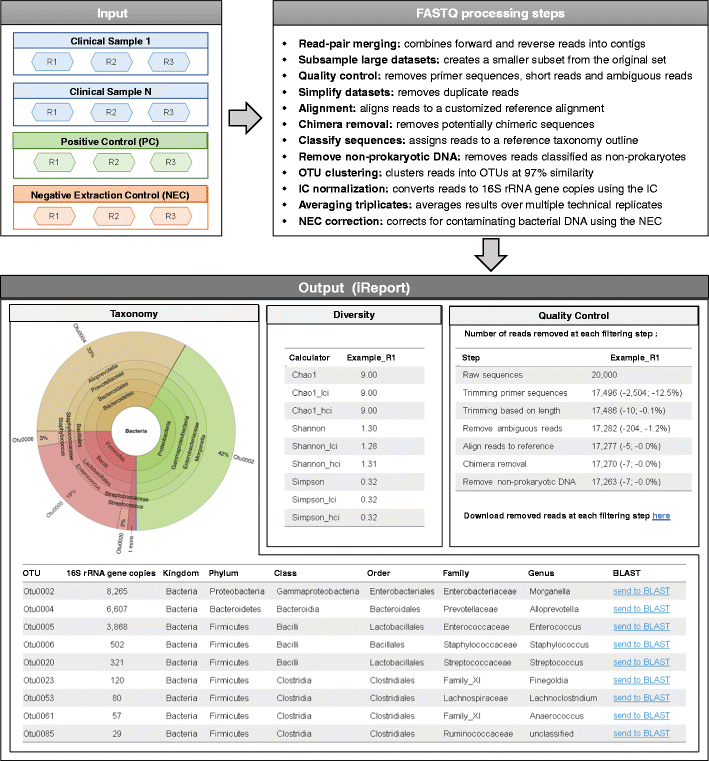
\includegraphics[scale=0.5]{chapters/images/mycrobiota/mycrobiota-fig1.png}
\caption{Schematical overview of the bioinformatics pipeline. FASTQ-formatted sequences obtained from triplicate experiments using micPCR/NGS (R1, R2, and R3) are automatically processed via the use of 32 (mothur) tools that have been integrated and combined in Galaxy as an “end-to-end” analysis service. The results obtained per sample (average of triplicate results) are presented to the user in a single, interactive iReport that consist of three tabs. The taxonomy tab visualizes and lists the resultant microbiota profiles. The diversity tab summarizes the results of three diversity calculators (Chao1, Shannon, and Simpson). The quality control tab provides an extensive overview of the quality control measurements during the analysis}
\label{fig:mycrobiota-pipeline}
\end{figure}


\section*{Results}

\section*{Discussion}

In this study, we developed and explored the utility of an “end-to-end” microbiota profiling platform (MYcrobiota)—consisting of our
previously published 16S rRNA gene sequencing methodology (micPCR/NGS) in combination with an easy-to-use bioinformatics pipeline—to
investigate human samples for the clinical diagnostic laboratories. The bioinformatics pipeline designed during this study allows for
a fully automated sequence interpretation of 16S rRNA gene NGS data that is obtained using the validated micPCR/NGS protocol without
the need for advanced bioinformatics skills that are often unavailable in the clinical diagnostic laboratories. The MYcrobiota results
are presented using (interactive) visualizations and tables, including an overview of all removed sequences during the analysis that
allows for a manual evaluation of the quality measurements pre-installed within the bioinformatics pipeline. Moreover, connections of
OTU representative sequences to the external NCBI database are available and can be used to ensure that the taxonomic identification
of bacterial genera is correct [16]. Importantly, the summarizing reports are relatively small in size, and storage of these files
enables the traceability of patient test results that are required for clinical diagnostic laboratories according to quality requirements.

Using MYcrobiota, we processed a total of 47 clinical samples and compared the results to routine bacterial culture. Our results showed
that the majority of bacteria identified with culture were also identified with MYcrobiota, but the majority of bacterial taxa identified
with MYcrobiota were not identified using culture. Many of the additional bacterial taxa identified using MYcrobiota are obligate anaerobes
that were commonly detected as a large component of the microbial population in samples obtained from damaged skin sites, which is consistent
with previous studies [17, 18]. Indeed, it is well known that anaerobic bacteria are able to cause serious and life-threatening infections
but are often overlooked due to their requirement for appropriate methods of collection, transportation, and cultivation [19]. Therefore,
the culture-free MYcrobiota detection platform can play an important role in the identification of the bacteriological etiology of anaerobic
infections or any other infections caused by fastidious microorganisms. Of note, it could be argued that the development of extensive culture
techniques (so-called culturomics) may eventually facilitate the successful culture of supposedly “non-culturable” microbial isolates [20].

In addition to the accurate detection and identification of bacterial OTUs within clinical samples, MYcrobiota also provides the relative
abundances in combination with the absolute abundances for each detected bacterial OTU. This feature allows clinicians to obtain a comprehensive
overview of the microbial composition of the clinical sample so that each quantified bacterial OTU, as well as the bacterial community as a whole,
might be taken into account in clinical decision-making. Additionally, MYcrobiota allows for the removal of contaminating DNA from environmental
sources in order to accurately and reliably investigate very low bacterial biomass, or no bacterial biomass, clinical samples [6]. For example,
MYcrobiota confirmed the absence of 16S rRNA gene copies in eight of the ten samples that generated culture-negative results. The two discrepant
samples contained either anaerobic bacteria or low amounts of the fastidious Kingella bacterium respectively. The ability to confirm culture-negative
results improves the reliability of culture-negative diagnostic results. Additionally, the ability of MYcrobiota to detect bacterial OTUs at very low
abundances makes MYcrobiota a suitable method to investigate normally sterile body sites, such as synovial fluids, cerebrospinal fluids, and blood samples.
It should be noted however that the authors are aware of the fact that the construction of MYcrobiota is only a first step in the transition of microbiota
research into actual clinical diagnostics. Extensive clinical and financial validation studies will be needed in order to validate and justify the routine
introduction of molecular microbiota profiling methods into clinical diagnostic laboratories.

In conclusion, the stepwise development of MYcrobiota paves the way to introduce quantitative microbiota profiling into the clinical diagnostic
laboratory. The method provides a highly accurate and comprehensive overview of the microbial composition of clinical samples or, alternatively,
confirms the absence of 16S rRNA gene copies in culture-negative samples, using a standardized and validated 16S rRNA gene NGS workflow. Despite
some shortcomings, e.g., lack of species identification and the inability to provide detailed information on antibiotic susceptibility, our data
illustrates that MYcrobiota has promising applications in the field of clinical diagnostics and warrants investment in future studies to accurately
evaluate the clinical relevance of 16S rRNA gene NGS results in clinical samples.

\section*{Notes}

\subsection*{Compliance with ethical standards}

An acknowledged national ethics committee from the Netherlands (Medisch Ethische Toetsingscommissie Noord-Holland, http://www.metc.nl) approved the
study protocol (M015–021), and all experiments were performed on leftover material of the included clinical samples in accordance with the relevant
guidelines and regulations. The national ethics committee waived the need for participant consent as all data were anonymized and analyzed
retrospectively under code.

\subsection*{Conflict of interest}

The authors declare that they have no conflict of interest.


\bibliographystyle{ieeetr}
\bibliography{references}
